\chapter{Coverage path planning problem} 


\minitoc

The following section is devoted to the Coverage Path Planning (named CPP). Until now, the work presented was focus on optimizing the position and orientation of a fix number of cameras to cover a vast and complex areas. 
The method introduced, use GA or a more flexible (but slower) GAPSO. These algorithms give an efficient result to estimate the pose of a set of fix cameras. To find a solution for the CPP problem we propose for the first time to use the algorithms developed for the cameras positioning to find the set of useful waypoints. Instead to use the conventional method based on sweep and spiral in simple polygon. The optimized poses of the cameras are considered as waypoints of a complete path. 
The detail of the proposed solution to optimize the CPP problem and few experiments made are presented in these sections.
 

\section{Sequential method} \label{sec:CPPsequantielMethod}
To optimize the CPP problems a simple and innovative method has been developed. The method proposed here can be decomposed in 3 principal parts all interconnected. 
\begin{itemize}
	\item Number of waypoints : 
	A crucial step is to estimate the number of waypoints. A wrong estimation of a too high or to low will cause a bad area coverage or a to complex computation.
	\item Waypoints positioning : 
	The waypoints positioning optimization is the more crucial step. As already discuses numerous solutions has been studied to optimize the pose of the cameras depending on several constraints. Based on it and the experiments made until now, an efficient algorithm has been chosen and adapted to pose estimate each waypoint (see Section  \ref{sec:hybridGAPSO}). 
	\item  Path plan computation : 
	 When the number and the position of the waypoints has been computed the last step is to find the shorter route  passing by all the waypoints. The route must start and finish at the same position (as for the TSP see Paragraph \ref{par:TSPPathPlan} and detailed in Section \ref{sec:TSP2}).
	
	% the number of waypoints will cause a  more complex and longer estimation of the pose for each of them and increase the complexity to compute a path. Otherwise with a too low number of waypoint the area will not be well cover and leave some black hole. 
\end{itemize}

The proposed method having the advantage to optimize independently all the waypoints and the path plan. This method is also not systematically based on sweep and allows to have a shorter path adaptedt to a complex map. Moreover the proposed CPP having with the same starting point and ending point. In practice the return to the starting point is meaningful. 


\subsection{Number of waypoints sestimation}\label{sec:NmbWaypoint}

It is difficult to estimate properly the minimum of waypoints which are necessary to cover a complex area.
To do so, a two-step procedure has been implemented. The procedure is based on the pose optimization for a fixed number of waypoints introduced in the precedent Chapter \ref{chap:waypointPoseExp}. 
The first step is to find the minimum number of waypoints depending on the area to cover like formulated in the
 Equation \ref{Eq:waypointN}. \\
\begin{equation}\label{Eq:waypointN}
\frac{ A_{room} - \sum_{i=1}^n A_{wall i} }{A_{cam}} \times \mbox{Threshold Rate} = \mbox{NWayPoint}
\end{equation}

\begin{itemize}
\item[-] $ A_{room}: $  area of the Room (length $\times$ width)
\item[-] $ A_{Wall}: $  area of the obstacle like wall (length $\times$ width)
\item[-] $ A_{Cam}: $   area cover by the camera in the maximum size of $z$
\item[-] $ \mbox{NWayPoint}: $  number of waypoints
\item[-] $ \mbox{Threshold Rate}: $ objective threshold rate 
\item[-] $S:$ one solution of waypoints set 
\item[-] $evalCost:$ cost function  
\end{itemize}

The second step is to compute GA optimization until the threshold is reached. At the convergence of each GA, if the threshold rate is not reached one more waypoints is added and a new GA optimization start with one more waypoints. The algorithm used to estimate the number of waypoints is explained in the "Algorithm 1 Estimation of the number of waypoints".  
               %  while increasing the number of waypoints like explained in the Algorithm 1 Estimation of the number of waypoints.  

\begin{algorithm}{}
\caption{Estimation of the number of waypoints}\label{alg:euclid}
\begin{algorithmic}[6]
\Procedure{NmbWaypoint}{$A_{room},A_{Wall},\mbox{Threshold Rate},A_{Cam}$}
 \State $S\gets 0$
  \State $NWayPoint\gets \frac{ A_{room} - \sum_{i=1}^n A_{wall i} }{A_{cam}} \times \mbox{Threshold Rate} 
 $  (Equation \ref{Eq:waypointN})
  \While{$eval Cost(S)\leq ThresholdRate$}
	 \State $S \gets GA(NWayPoint)$
	  \State $NWayPoint\gets NWayPoint+1$
  \EndWhile\label{endwhile}
\State \textbf{return} $NWayPoint$
\EndProcedure
\end{algorithmic}
\end{algorithm}

At the end of these steps, we have the number and a good set of waypoints poses from the last GA convergence. The waypoints poses can directly be used, but can also be refined using the adapted PSO (as in the GAPSO see \ref{sec:hybridGAPSO}). Once the number and the efficient poses of the waypoints founded the next step is to compute the path planning. The path planning has to pass by all the waypoints found before to return to the starting point.  
%%%%%%%%%%%%%%%%%%%%%%%%%%%%%%%%%%%%%%%%%%%%%%%%%%%%%%%%%%%%%%%
%%%%%%%%%%%%%%%%%%%%%%%%%%%%%%%%%%%%%%%%%%%%%%%%%%%%%%%%%%%%%%%%%%%%%%%%%%%%%%%%%%%%%%%%%%%%%%%%%%%%%%%%%%%%	
	
% \begin{mfigures}[!]{optimisation of the path plannig}{fig:Path_planning} \centering
%\mfigure{width=.4\linewidth}{img/22pts_WaypointsDijktra2.jpg}{Poses of every image captured in the room.}{subfig:Dijktra}
%\hspace{1cm}
%\mfigure{width=.4\linewidth}{img/22pts_WaypointsGA2.jpg}{Path compute with Dijktra multi goal.}{subfig:GATSP}
%\end{mfigures} 
 
  \subsection{Sorted waypoints and path planning.} \label{sec:sorted}
In the previous section, the method to obtain the list of waypoints positions to have a desired coverage has been detailed. The list of waypoints has to be sorted, in order to compute an efficient path with the shorter travelling distance passing by all the waypoints. In order to create an efficient path passing by all optimised waypoints the problem is formalized as a TSP. The TSP was quickly introduced in the Paragraph \ref{par:TSPPathPlan} and more detail about is provided in the following sub-section.

% \subsubsection*{a)}{Shortest Path Problem}
% \\Normally, finding a shortest path between two points in configuration space is mature enough. In our case we assume the waypoints as multi goals. So the planning in this method will simply find at every waypoint the shortest Euclidean distance from the other available non-traversed waypoints. Based on that a ranked waypoints list will be generated. This will not guarantee a globally shortest distance, but will only choose the shortest distance every time a waypoint is visited.
 
\subsubsection*{Traveling Salesman Problem. }\label{sec:TSP2}

%%%%%%%%%%%%%%%%%%%%
% \begin{figure}[htp]
%   \centering
%   \subfloat[Image d'origine]{\label{fig:edge-a}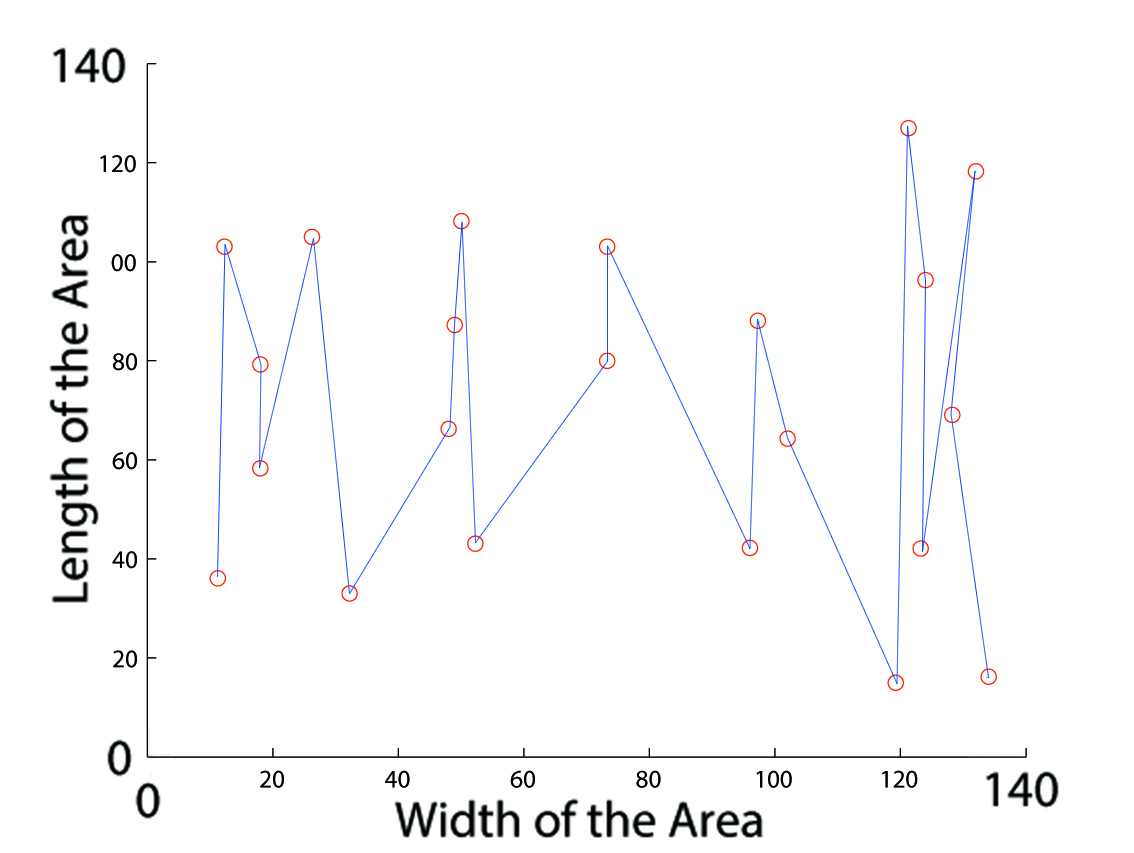
\includegraphics[scale=0.75]{22pts_WaypointsDijktra2.jpg}}
%   \hspace{5pt}
%   \subfloat[Après une détection des contours de Laplace]{\label{fig:contour-b}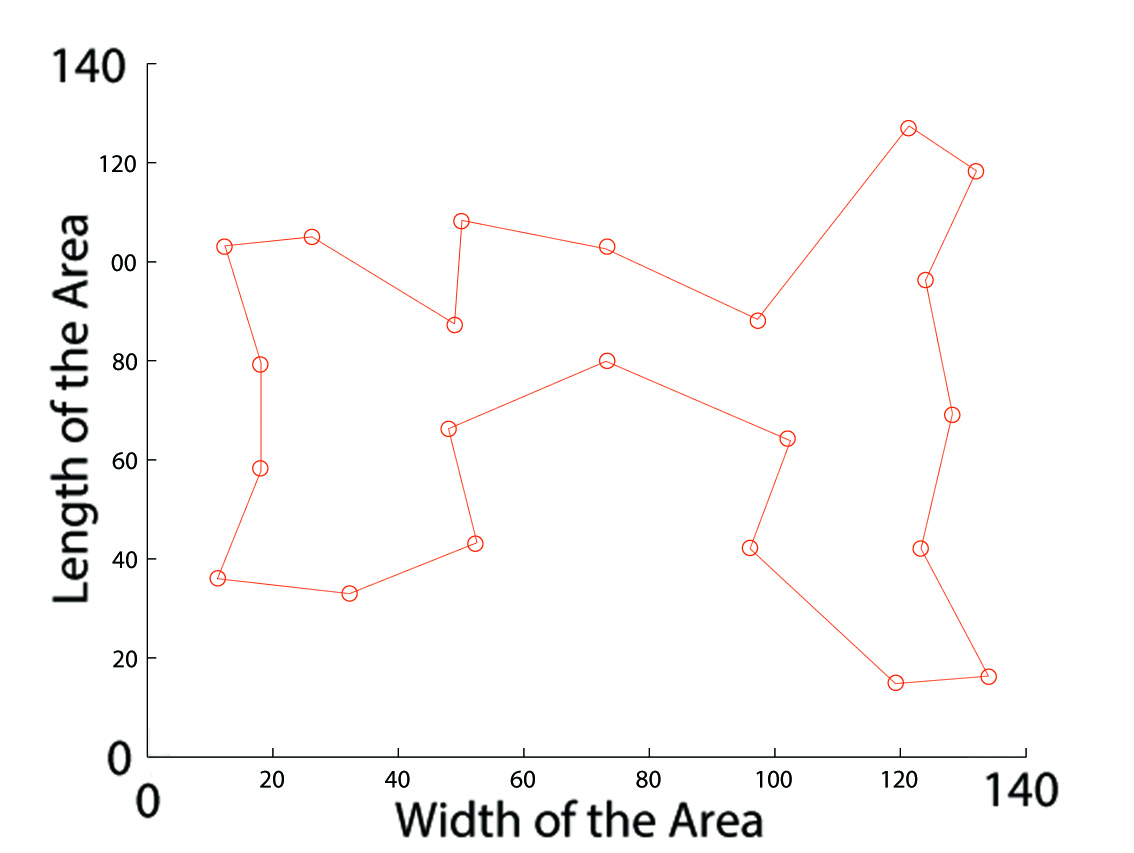
\includegraphics[scale=0.75]{22pts_WaypointsGA2.jpg}}
%   \label{fig:contour}
% \end{figure}
%%%%%%%%%%%%%%%%%%%%

\begin{mfigures}[!]{Optimization of the path planning.}{fig:Path_planning} \centering
\mfigure{width=.4\linewidth}{img/fig5-a.png}{Every pose after the optimization of the waypoint positioning. }{subfig:Path_planning1}
\hspace{1cm}
\mfigure{width=.4\linewidth}{img/fig5-b.jpg}{Path compute with GA multi objective for TSP.}{subfig:Path_planning2}
\end{mfigures}	

The sorted path can be formulated as Travelling Salesman Problem (TSP). To remember the TSP is inspired by a question asked by a salesman "\textbf{What is the shortest path passing by each city only one time and return to the starting city? When i know a list of cities and the distances between each pair of cities.}". The TSP problem is a well known NP-Hard and NP-complete problem (see \citep{236*karp1972}) and different solutions exist to optimize it depending of the context. 
Ponnambalam et al 172* \cite{172*ponnambalam2004} propose using a multi-objective GA to optimize the TSP. Moreover then, the GA used Ponmambalam et al 172* \cite{172*ponnambalam2004} provide the GA set-up (the mutation rate, population size,...). DAVIES et al \cite{56*davies2006} propose also to use the GA to solve the TSP applied on robotic with obstacles constraint. \\
Based on the literature, GA since adapted and efficient enough to optimize the TSP problems.
The GA has to be set-up properly depending then the specific TSP problem. The GA set-up was discussed in the Section \ref{sec:Setting and set-up}. The know the more appropriate set-up to optimize the TSP, several studies has been made  as \citep{68*muhlenbein1989,80*serpell2010,139*razali2011} 139*. The conclusion of these studies is to use a simple GA for combinatory problem. That mean the operator has to be adapted (using swap for example) with a high mutation rate and a very elitist selection.
To illustrate the GA ability one example using an adapted GA (high mutation rate,  elitist selection and combinatory formulation) solution is provided in the Figure \figref{fig:Path_planning}.



%\texttt{\begin{figure}[t!]
%  \centering
%   \subfloat[ Every pose after the optimization of the waypoint positioning.  ]{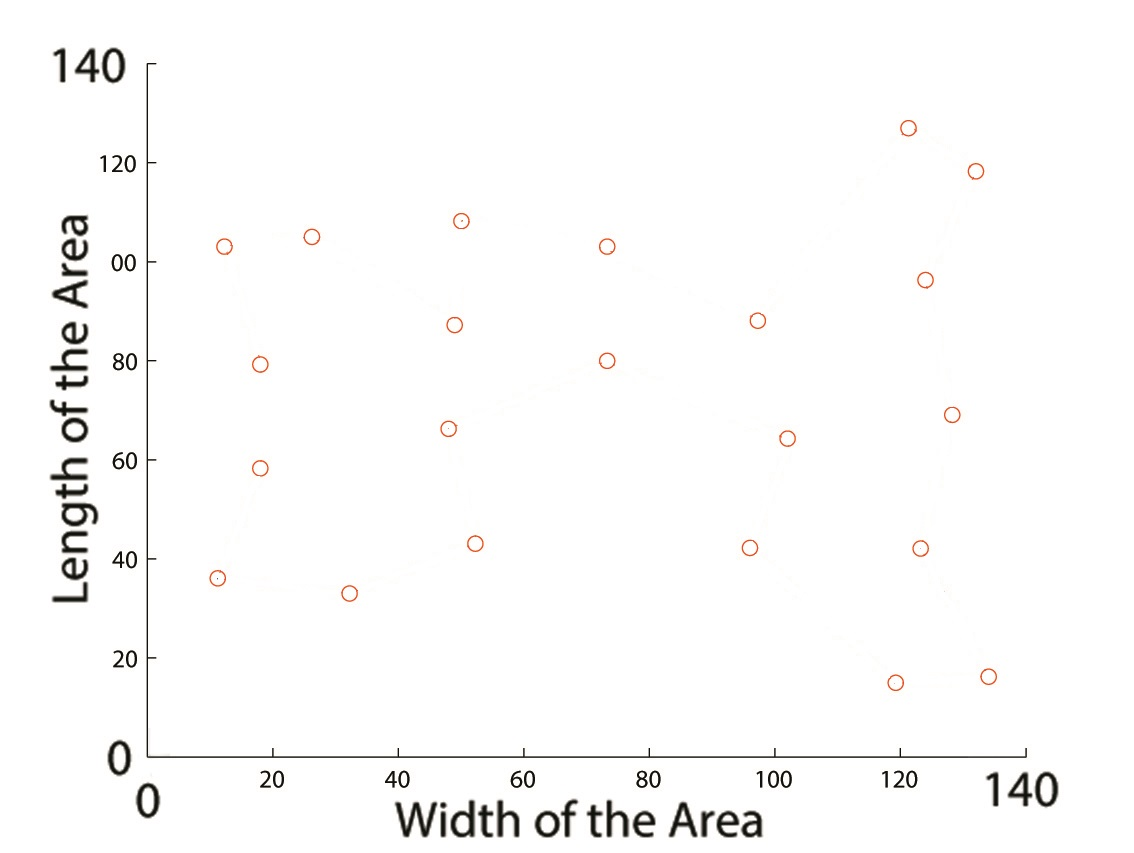
\includegraphics[width=0.45\textwidth]{fig5-a.png}}
%   \hfill
%   \subfloat[Path compute with GA multi objective for TSP. ]{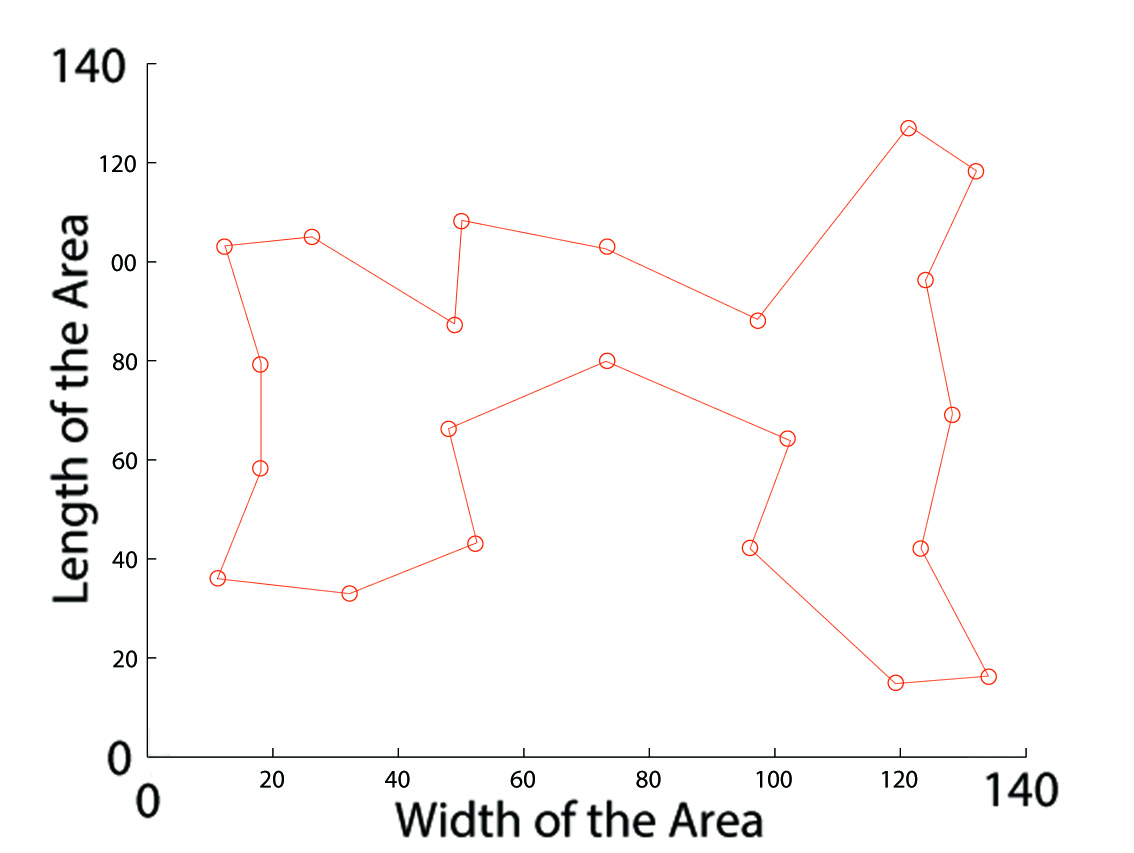
\includegraphics[width=0.45\textwidth]{fig5-b.jpg}}
%  \caption{Optimization of the path planning.}\label{fig:Path_planning} 
%\end{figure}}
% Every node which is a point in space is represented as a city and the Euclidean distances between the cities are calculated and used as a cost function. The path is organized based on the minimum distance traversing over all the cities (or waypoints). To find an optimized solution GA is here again used.

% The privilege of TSP problem formulation and solving it using GA over the other shortest path algorithms like Dijkstra, is that it provides global  complete solution traversing all the waypoints not finding a path from a starting node  to a goal node. The GA approach is more clarified and discussed by Trevor \textit{et al}     \cite{GA_Path}. 
%  The distance covered by a path that is planned by GA is 513 meters, which is shorter by the factor of 1.8 compared to the distance covered by Dijsktra multi goal approach which is 963 meters. Using the GA  to optimize  the scheduling problem of waypoint makes a more efficient result and especially the GA unlike the Dijsktra multi goal, it is more efficient to sort a high number of waypoints.\\ 
 
\subsubsection*{Complexity of trajectory. }\label{tarjectory}

Once the waypoints position estimated and the shorter path passing by all the waypoints computed it is interesting to can evaluate the trajectory complexity. The trajectory complexity can be a great clue of the path reliability.  It also be useful to compare our solution to the more classical sweep trajectory.
 
To estimate the trajectory, two indicators are used to evaluate properly the path complexity. The first indicator is the distance of the trajectory. The distance allows to evaluate basically the optimization of the path planning. This indicator is directly included in the optimisation process as discussed before (see Section \ref{sec:TSP2}). 
Evaluate the trajectory only by using the distance indicator is not enough and another indicator must be associate to can evaluate quickly the trajectory complexity. To estimate the complexity in terms of curve for the UAV evolving in the 3D space the angles at each node is studied. 
The complexity of trajectory indicator is computed as follow: 
\begin{equation}\label{Eq:trajectory}
\mbox{Trajectory complexity}=\frac{ \sum_{i=1}^{size(\alpha)} 180- \alpha_{i}  }{size(\alpha)}   
\end{equation}
Where $\alpha_i$ is an angle of curve in the trajectory as in Figure \figref{fig:trajectoirAlpha}. \\
$Size(\alpha)$ is the number of curve in all the trajectory.\\ 
This method can give an idea of the global trajectory complexity despite this simplicity. 
The two indicator presented (the distance and the trajectory complexity) are used during the next section to evaluate the gain of the proposed method.
	
 \begin{mfigures}[!]{optimisation of the path plannig}{fig:trajectoirAlpha} \centering
\mfigure{width=.4\linewidth}{img/TrajectoirAlpha3.png}{Extraction of the curve angle in the trajectory.}{subfig:trajectoirAlpha}
\end{mfigures} 
%%%%%%%%%%%%%%%%%%%%%%%%%%%%%%%%%%%%%%%%%%%%%%%%%%%%%%%%%%%%%%%%%%%%%%%%%%%%%%%%%%%%%%%%%%%%%%%%%%%%%%%%%%%%%
	
	
				



%%%%%%%%%%%%%%%%%%%
			\section{Experiments} \label{sec:experiment}

The method proposed optimizing the CPP problem is tested during different experimentations. The experimentations brings out the advantage and the limit of the developed method. The experiments are structured in sub-section with show the method and algorithms in more and more complex experimentations.

\subsection{Rectangle obstacle} \label{experiment}

 \begin{mfigures}[!]{optimisation of the path planing}{fig:final_room2} \centering
%\mfigure{width=.4\linewidth}{img/room_python.PNG}{Poses of every image captured in the room}{subfig:RoomPy}
\mfigure{width=.4\linewidth}{img/room_full.png}{Room Coverage}{subfig:fullRoomPath}
\hspace{1cm}
\mfigure{width=.4\linewidth}{img/VrepMyOptimization.png}{Pose of every images with the path planning}{subfig:PathPlanning}
\mfigure{width=.4\linewidth}{img/VrepCellDecopo1.png}{Room in V-rep}{subfig:VrepCellsDecomp}

\tabsVrepPath
\end{mfigures} 

In order to experiment the proposed method for CPP a simple indoor experiment is proposed to begin.
The experiment proposed is based on the one discussed previously on Section \ref{sec:expRectObstacle}.
To remind the experiment is made in a simulated room ($15 \times 14 m^2$). The area to cover is shown in the Figure \figref{subfig:fullRoomPath}. The camera parameter are the same, $4 \times 3 m^2$ when $z$ is equal to one and the $z$ factor can be equal at $[0.5;1;1.5]$. On the other hand, the sweep is computed with the camera at the maximum altitude to have the biggest area coverage possible.

Thanks to this first experiment the path planning proposed appear much more appropriate (see Figure \figref{fig:final_room2}). The path planning obtained by our method proposed a shorter path, 881.6 pixel length when  the path by sweeping is at 1137 pixel length. The path proposed by the sweep is longer notably due to the return to the starting point, but not only. The junction between the start and finish of the swept path is 245 pixel long, with mean the path useful to fully cover the area is around 892 pixel long. Moreover the proposed path planning in addition then the shorter path proposes also a better trajectory complexity  with 65.22$^\circ$ instead to 97.81$^\circ$ for the path with sweep.
Finally the proposed solution allows a better path planning thanks to this optimized waypoints. Despite a better path plan efficiency few points ($g_i$) in the area are not covered in contrary than the traditional swept method.



\subsection{Using Mask to describe area.}\label{coverageOutDoor}

The gain for the indoor area is important. The gain is mostly due to the well optimised position of the waypoints. The experiment must be extended for a bigger and complex area with a higher coverage rate requirement.


\subsubsection{Vast and complex area.} \label{fey_map_CPPP}
 
 \begin{mfigures}[!]{Experimentation of coverage path planning in the outside area.}{fig:FleyPathPlan} \centering
%\mfigure{width=.4\linewidth}{img/room_python.PNG}{Poses of every image captured in the room}{subfig:RoomPy}
\mfigure{width=.4\linewidth}{img/fig10-a2.png}{Path planing using the pattern method.}{subfig:FleytfullRoomPath}
\hspace{1cm}
\mfigure{width=.4\linewidth}{img/fig10-b2.png}{80 waypoints for 98.28\% of coverage.}{subfig:FleyPathPlanning}
\mfigure{width=.4\linewidth}{img/fig10-c2.png}{Path with 80 waypoints for a distance of 4015.6 px.}{subfig:FleyPathPlan}

\tabsimuposeFleyPath
\end{mfigures} 
 
 
% \begin{figure}[t!]
%  \centering
%   \subfloat[Path planing using the pattern method.]{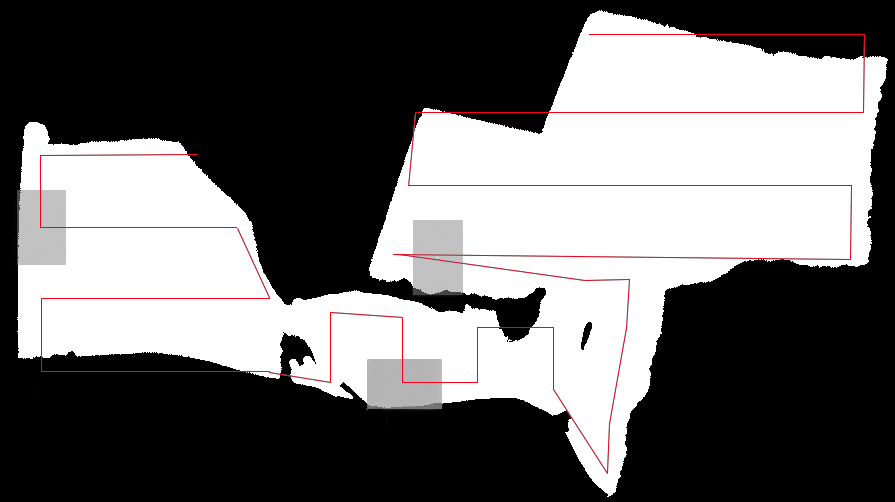
\includegraphics[width=0.475\textwidth]{fig10-a2.png}}\qquad
%   \subfloat[80 waypoints for 98.28\% of coverage.]{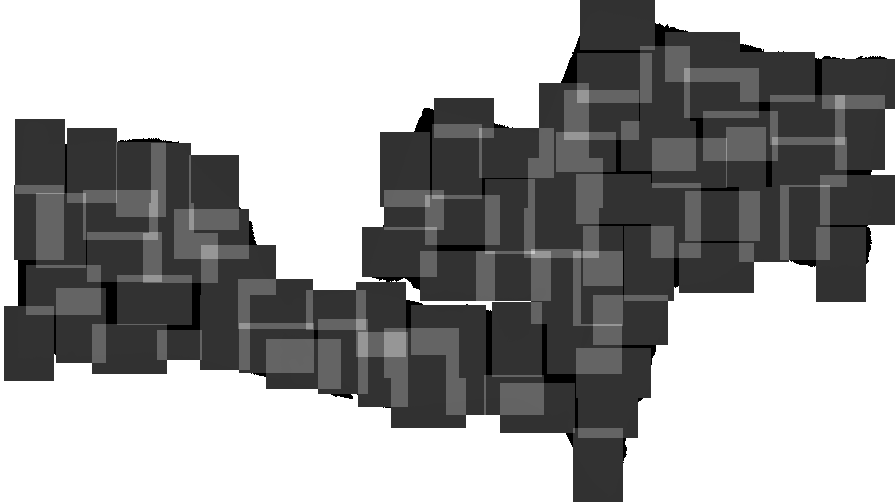
\includegraphics[width=0.475\textwidth]{fig10-b2.png}}\hfill %zcalvisson2result1cout_94_862284_gen_3634_Ncam_110
% %\subfloat[Path with 110 waypoints for 94.86\%  ]{\includegraphics[width=0.55\textwidth]{fig10-c.jpg}}%zGAevolvTurnComplexCross_919Mut_001pop100cout_94_862284_gen_3634_Ncam_110Sorted  width=0.45
% \hfill %zcalvisson2result1cout_94_862284_gen_3634_Ncam_110
% \subfloat[Path with 80 waypoints for a distance of 4015.6 px. ]{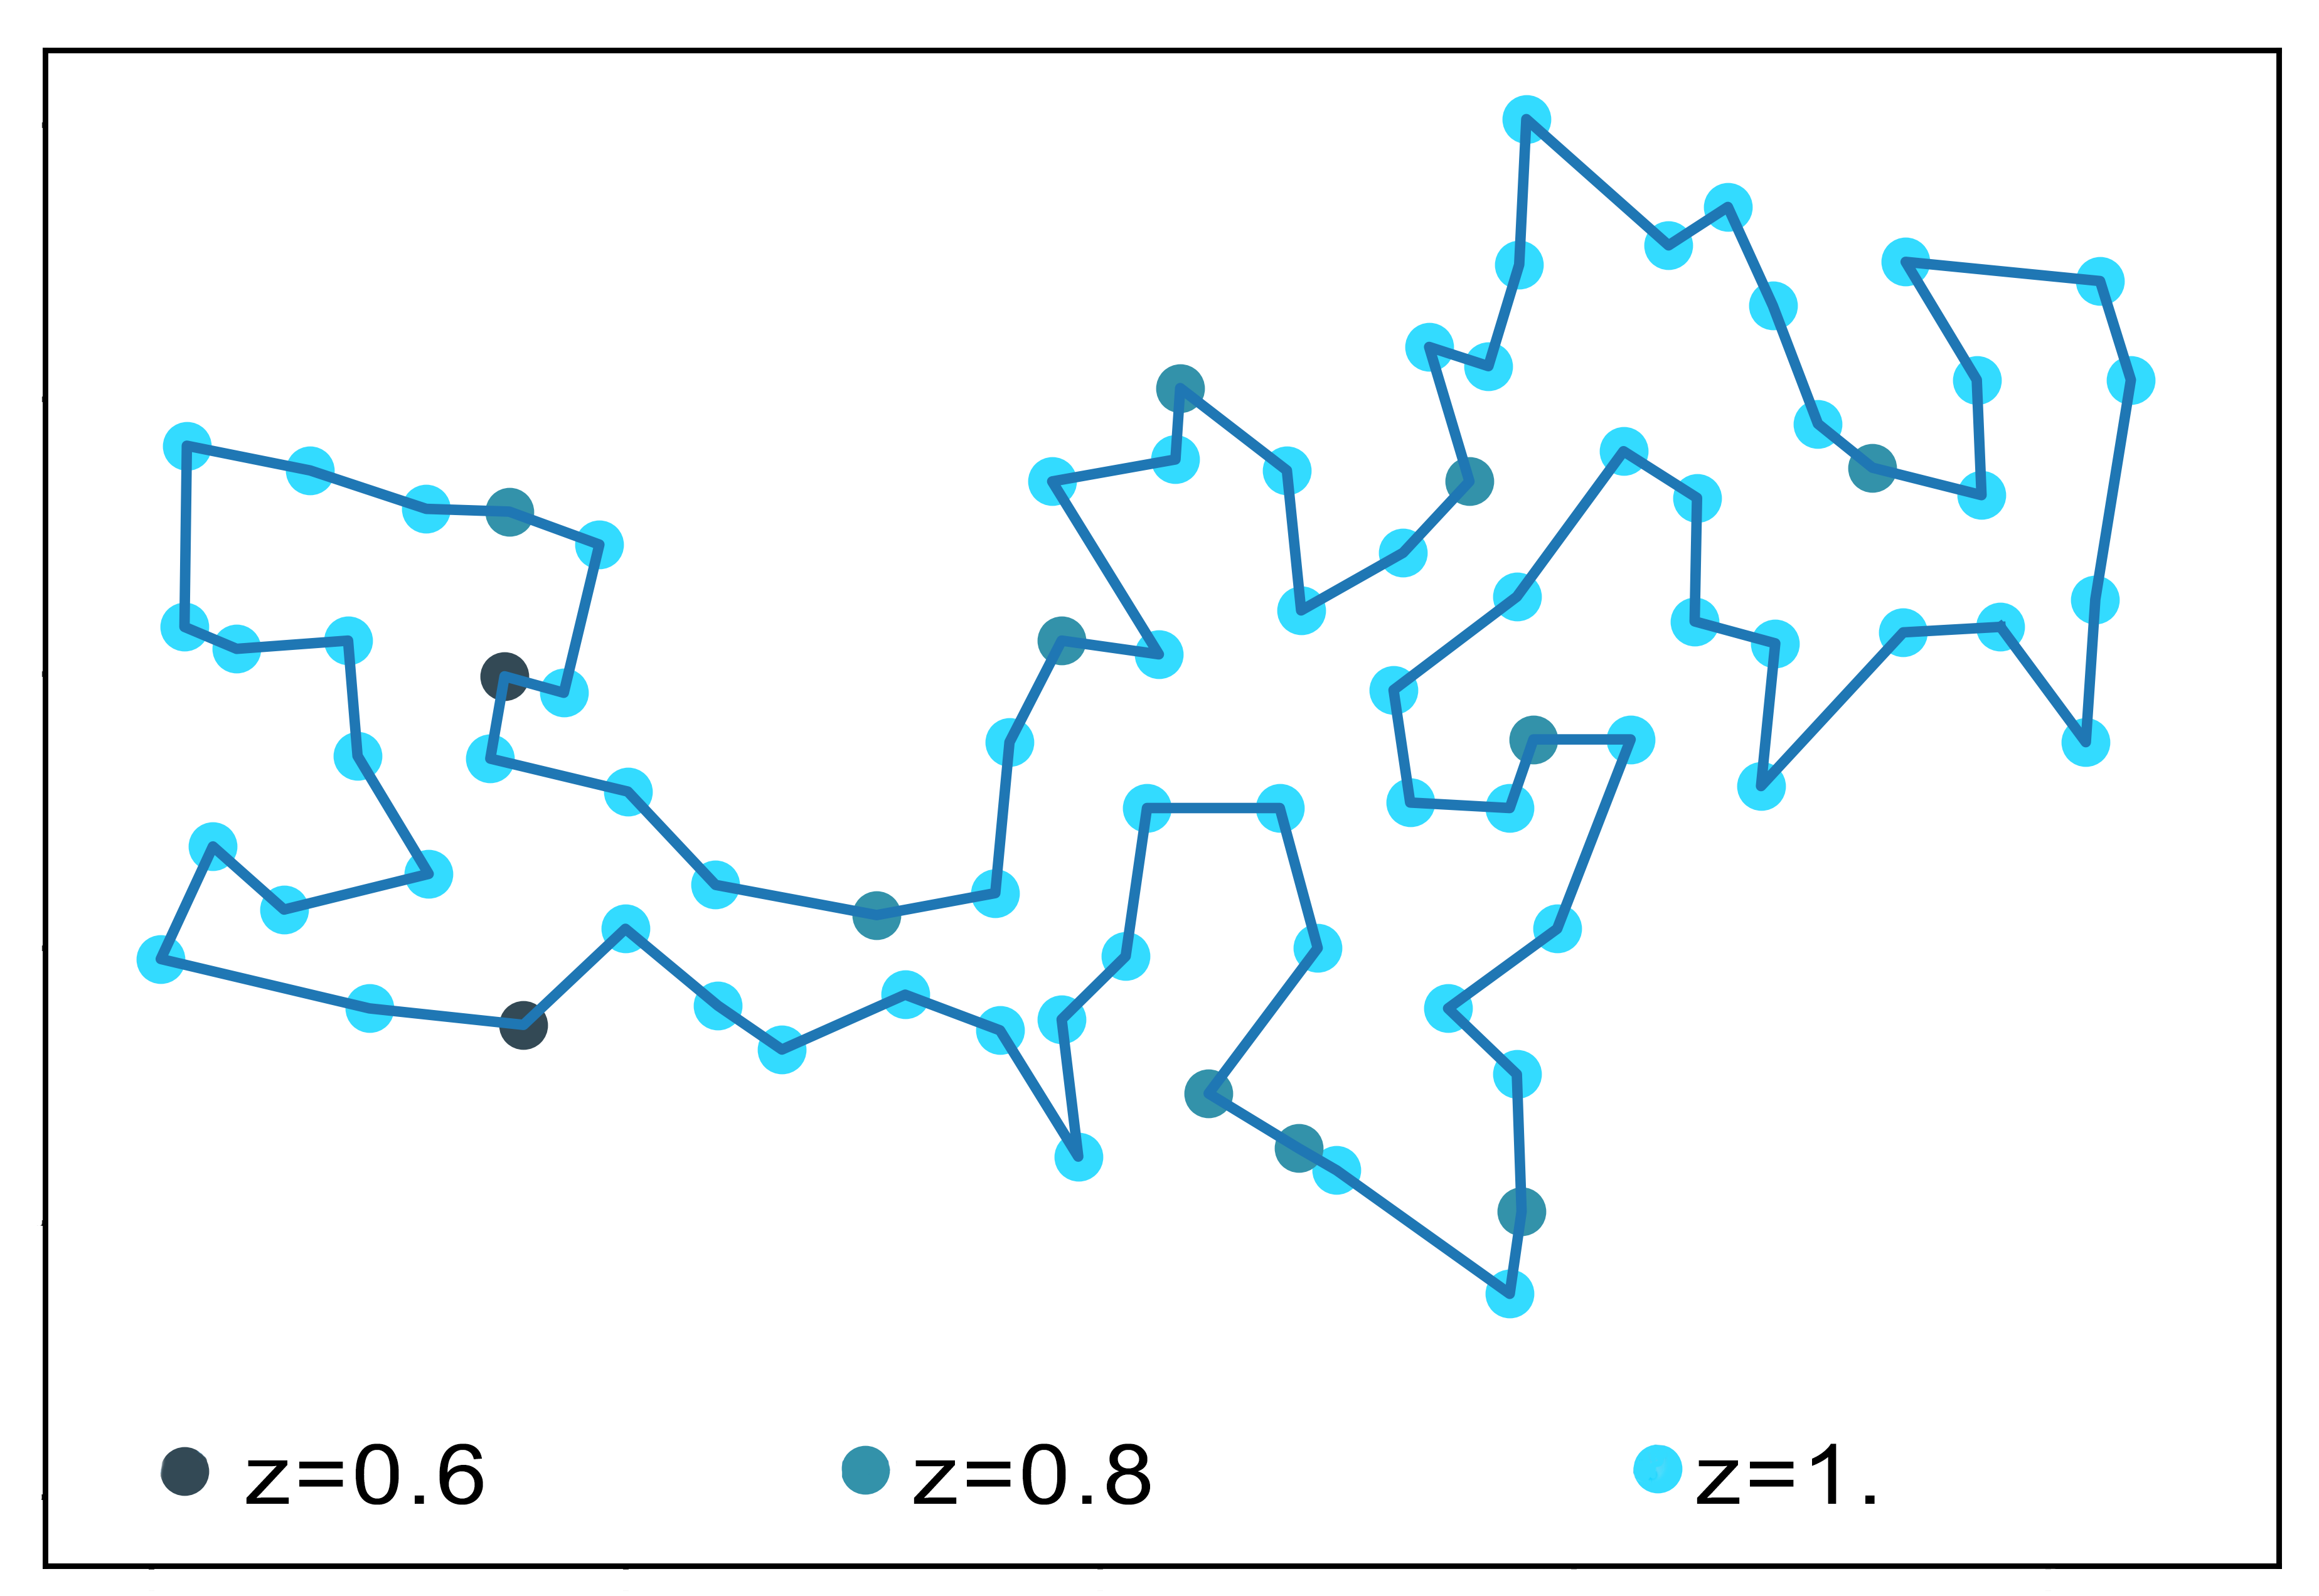
\includegraphics[width=0.45\textwidth]{fig10-c2.png}} \hfill
% \subfloat[][]{\tabsimupp}
%  %zcalvisson2result1cout_94_862284_gen_3634_Ncam_110
% %\subfloat[Path with 110 waypoints for 94.86\%  ]{\includegraphics[width=0.45\textwidth]{fig10-d_bis.jpg}}
%  \caption{Experimentation of coverage path planning in the outside area.}\label{fig:trajectoryPath} 
%\end{figure}

%\begin{table}[]
%\centering
%\caption{Outdoor simulation with path planing (Figure \ref{fig:trajectoryPath})}
%\label{pathPlan}
%\begin{tabular}{l|ll}
%\textbf {Parameters }             &\textbf{Value }                              &  \\ \cline{1-2}
%\cellcolor[HTML]{FFFFFF}{$z$}        & \cellcolor[HTML]{FFFFFF}{[}1;1,5;2{]}        &  \\
%\cellcolor[HTML]{F2F2F2}$\gamma$        & \cellcolor[HTML]{F2F2F2}portrait or landscape &  \\
%\cellcolor[HTML]{FFFFFF}Coverage & \cellcolor[HTML]{FFFFFF}waypoint snap        &  \\
%\cellcolor[HTML]{F2F2F2}Maximum size of camera projection & \cellcolor[HTML]{F2F2F2}70x105px             & 
%\end{tabular}
%\end{table}
%\begin{table}[]
%\centering
%\caption{Outdoor simulation with path planing(Figure \ref{fig:trajectoryPath})}
%\label{tab:pathPlan}
%\begin{tabular}{l|ll}
%\textbf {Parametres }             &\textbf{Value }                              &  \\ \cline{1-2}
%\cellcolor[HTML]{FFFFFF}{$z$}        & \cellcolor[HTML]{FFFFFF}{[}1;1,5;2{]}        &  \\
%\cellcolor[HTML]{F2F2F2}$\gamma$        & \cellcolor[HTML]{F2F2F2} portrait or landscape &  \\
%\cellcolor[HTML]{FFFFFF}Coverage & \cellcolor[HTML]{FFFFFF} stream record        &  \\
%\cellcolor[HTML]{F2F2F2}Maximum size of camera projection & \cellcolor[HTML]{F2F2F2}70x105px             & 
%\end{tabular}
%\end{table}
The CPP and more precisely the path planning part is compared to a standard method (the sweeping). We compare the CPP  in term of coverage, path plan distance and trajectory complexity. The standard method used for CPP uses an adapted pattern to cover an area. The patterned method application is based on several articles as \citep{144*torres2016,191*di2016,63*chao2008,66*galceran2013} 119* (see Section \ref{sec:CPPcellDecompSol}). %pattern155*

To focus on a bigger area the experiment for outdoor waypoints positioning in vast and complex area using  a mask  is reused as in Section \ref{sec:fey_map}. This experiment has the advantage to be vast and complex enough for the comparison between the sweeping method and the proposed method.\\
To compute the sweep, the area is firstly decomposed in cells to apply an appropriate sweep. In the second time the appropriate sweep are placed in each cells. The size of the sweep has been designed for the fix altitude depending then the size of the camera projection on to the floor at the highest altitude spite the resolution. 
The path plan using a sweeping method is visible in the Figure \figref{subfig:FleytfullRoomPath}. In order to cover completely the area several overlap and un-interesting region (the black region in Figure \figref{subfig:FleytfullRoomPath}) has to be covered too. 

The solution proposed by optimizing in a first time the waypoints position and in second time the path passing by the waypoints is applied. The optimization is made for a set of 80 waypoints which must cover over the 98\% of the area. This threshold is reached after a 3101 generations (see in \figref{subfig:FleyPathPlanning}). Once the waypoints optimized (in $x;y;z$ and roll) the path plan is computed using the method based on the TSP (presented in the Section \ref{sec:TSP2}). The final CPP is visible in the Figure \figref{subfig:FleyPathPlan} with the different altitude represented in color.

One more time and despite the increased size and complexity of the map (with increase greatly the complexity and the number of the waypoints optimization) the proposed solution give a better result. The path plan is shorter 4362px for the pattern method versus 4015px for our method. The path is also  easier to compute  in term of trajectory 82.14$^\circ$ versus 65.78$^\circ$.
In fact the optimization of the waypoints despite a not completely covered area offer good waypoints for the path planning. In fact the coverage rate over the 98\% of coverage can be considered more then enough depending then the application.
% The path proposed is established in the area to cover and the camera FoV. The pattern is adapted depending on the shape of the area and the size of the camera projection in order to have full coverage with the minimum of overlapping. The final path using the pattern method showed in Figure \figref{subfig:FleytfullRoomPath}.
 %\\ The solution proposed  establishes a path apparently more complex (see Figure \ref{fig:trajectoryPath}c) using the third dimension with a coverage rate somewhat lower, 98.28\% of coverage for the full area after 3101 generation.
% Although the distance of the path and the complexity trajectory based on Eq.(\ref{Eq:trajectory}) prove the efficiency of this method by a shorter distance and a better complexity indicator as depicted in Table \ref{table:trajectory}.\\
  
% \begin{table}[t]
%\begin{tabular}{|p{1.5cm}|p{1.8cm}|p{1.8cm}|p{1.8cm}|}
%  \hline
%   &Coverage rate & Path length (in px) & Trajectory complexity (Eq.\ref{Eq:trajectory})  \\  \hline
%  Pattern Method &  100\% & 4362.66 &82.14 \\ \hline
%  Ours Method &  98.28\% & 4015.6 &65.78 \\ \hline
%\end{tabular}
%\caption{Comparative table  of path distance and complexity.}\label{table:trajectory}
%\end{table}
%
%

%\begin{figure}[t]
%  \centering
%  \hspace*{\fill}
%  \subfigure[]{\label{subfig:satimg+mask}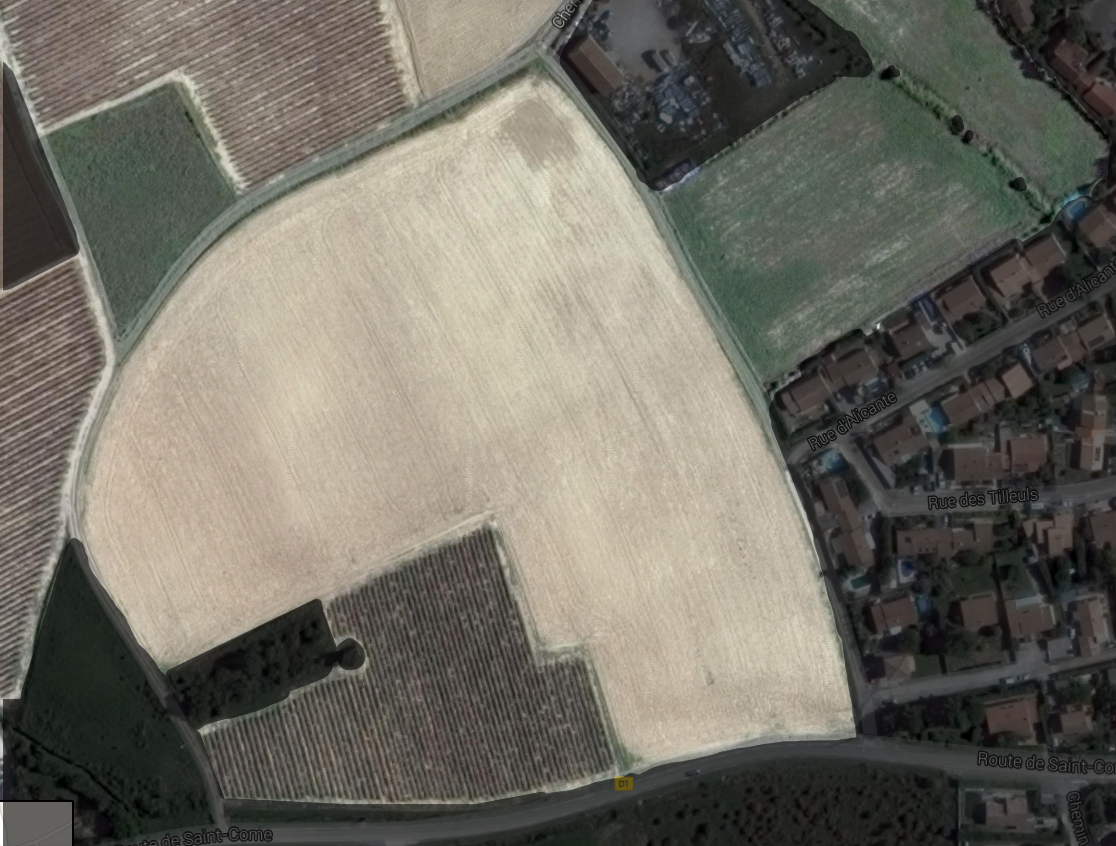
\includegraphics[width=0.48\linewidth]{calvisson2+mask.png}} \hfill
%  \subfigure[]{\label{subfig:satimgMask}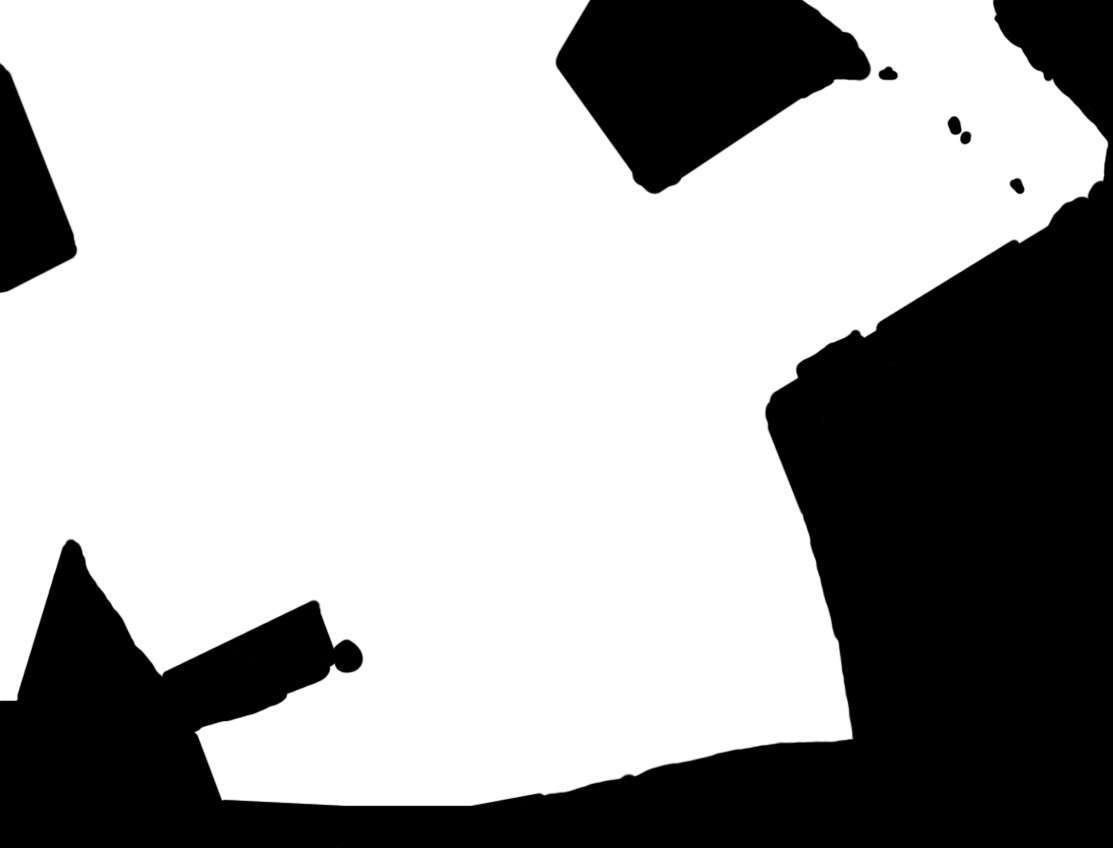
\includegraphics[width=0.49\linewidth]{calvisson2mask.png}}
%  \hspace*{\fill}
%  \\
%   \hspace*{\fill}
%  \subfigure[]{\label{subfig:satimgcoverage}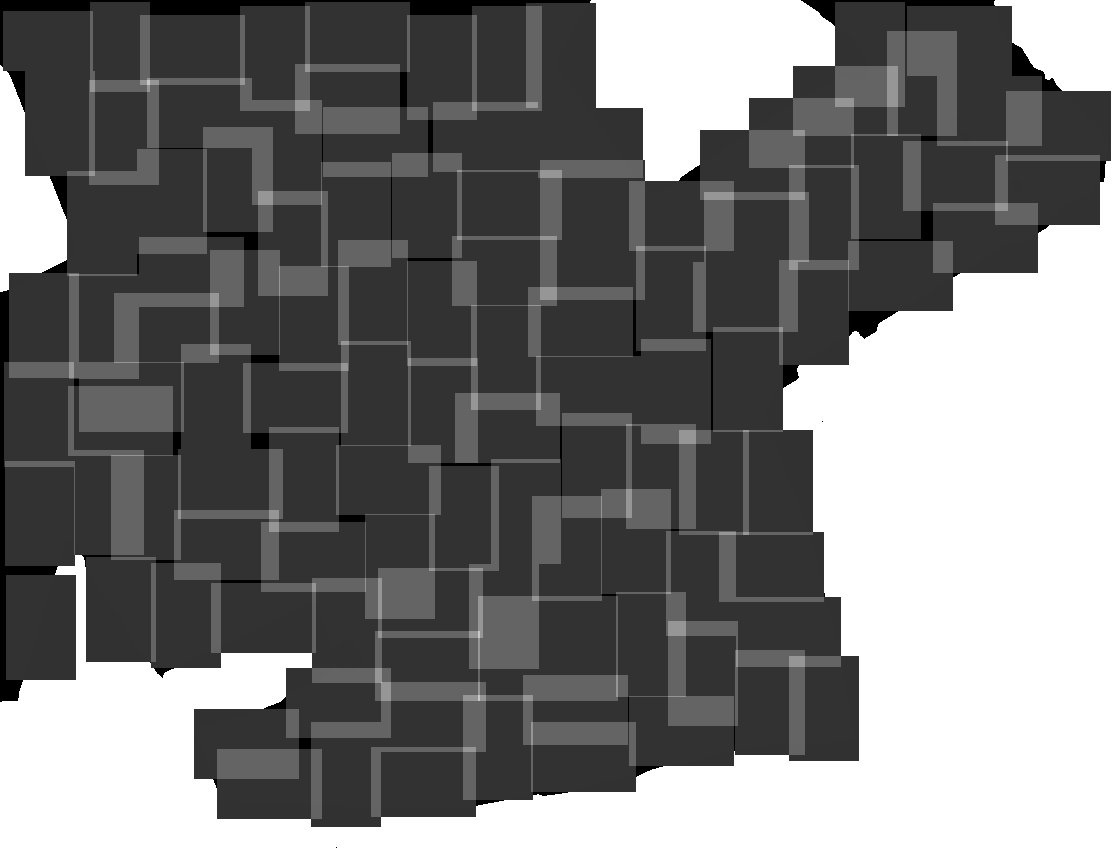
\includegraphics[width=0.80\linewidth]{zcalvisson2result1cout_98_260375_gen_170501_Ncam_110.png}}
%  \hspace*{\fill}
%  \hspace*{\fill}
%  \subfigure[]{\label{subfig:satimgNoncover}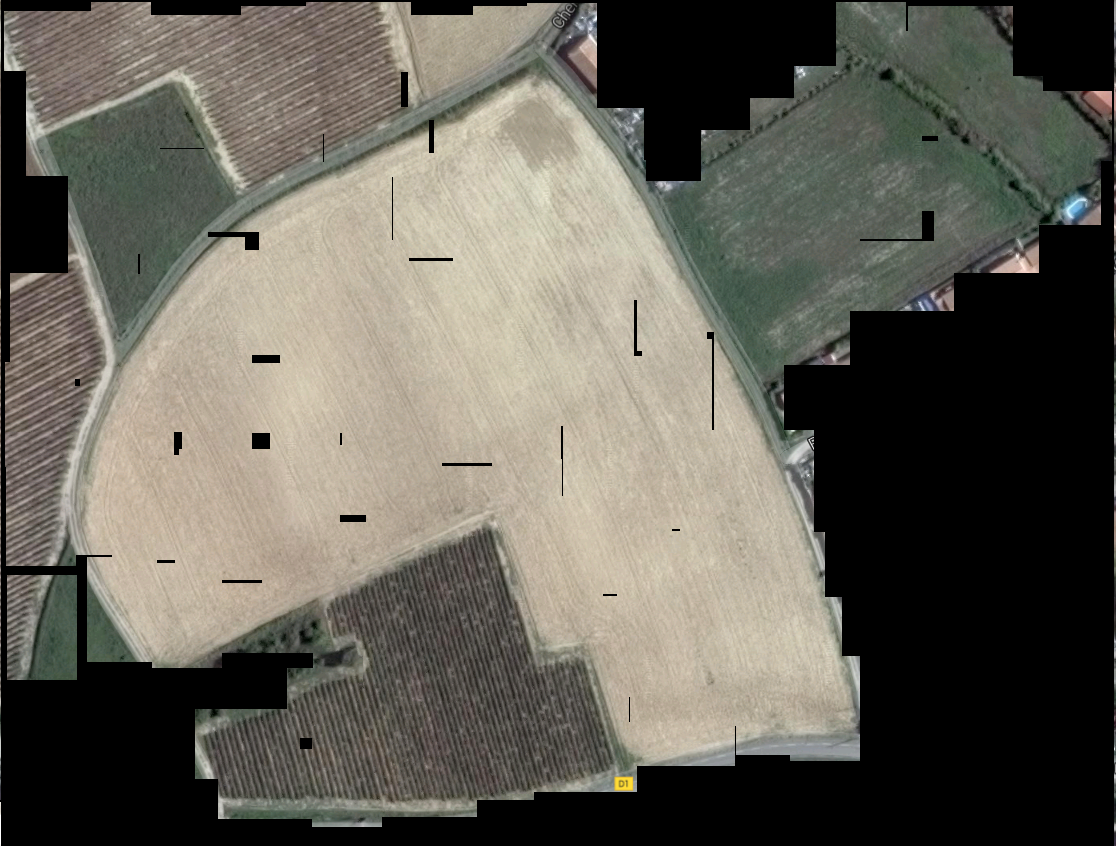
\includegraphics[width=.8\linewidth]{calvisson3cover.png}} \hfill
%  \hspace*{\fill}
%  \caption{ Optimization of the waypoint pose with a big outside area: (a) is the area to cover take form a satellite images,(b) is a mask of the area to cover, (c) is a result of the coverage with the waypoint position, (d) is the representation of the black hole.}
%  \label{fig:Rooms_shapes}
%\end{figure}



\subsubsection{Biggest map with numerous waypoints}
 
 \begin{mfigures}[!]{Experimentation of coverage path planning in the outside area.}{fig:CalvissonPathPlan} \centering
%\mfigure{width=.4\linewidth}{img/room_python.PNG}{Poses of every image captured in the room}{subfig:RoomPy}
\mfigure{width=.4\linewidth}{img/calvisson2maskPath2.png}{Path planing using the pattern method.}{subfig:CalvissonfullRoomPath}
\hspace{1cm}
\mfigure{width=.4\linewidth}{img/zcalvisson2result1cout_94_862284_gen_3634_Ncam_110.png}{110 waypoints for 94.862\% of coverage.}{subfig:CalvissonPathPlanning}
\mfigure{width=.4\linewidth}{img/CalvissonsizeWaypointPath.png}{Path with 80 waypoints for a distance of 4015.6 px.}{subfig:CalvissonPathPlan}
\tabsimuposeCalvissonPath
\end{mfigures} 

To continue the experiment a biggest area can be selected with require much more waypoints. The big area selected for test the coverage path planning is the same area then in Section \ref{sec:biggestMapcalWaypoint}. 
%The experiment is made on a bigger area to show the optimization efficiency despite the increaser number of dimension to optimize. 
The simple sweep path is computed based on the camera projection at the highest altitude (see in Figure \figref{subfig:CalvissonfullRoomPath}). Our method is computed  with 110 waypoints to estimate the poses. After 3634 generation for a coverage area at almost 95\% (see Figure \figref{subfig:CalvissonPathPlanning}) the path  can be computed (as explained in the section \ref{sec:sorted}).  The final CPP is shown in the Figure \figref{subfig:CalvissonPathPlan}. 

The solution proposed give a shorter path compare than the swept method (8173px versus 8582px) for a high level of waypoints coverage. But the difference between the 2 paths are not so important  %even more considering the  return to the starting point to the swept method (around 770px)
in term of distance. But the difference of trajectory complexity gives an important advantage of the method proposed.\\
Thanks to this experiment the limit of our method begins to appears. The principal limitation is due to the difficulty to optimize numerous waypoints (as that was discussed in the Section \ref{sec:biggestMapcalWaypoint}). The increased number of waypoints associate to a high level of coverage rate required, push the GAPSO optimization to the limit. Numerous generation are necessary before to converge. On the other hand, the path plan computation appear efficient despite the increased number of waypoints and globally the solution proposed give a better CPP in term of distance and trajectory complexity for a high coverage rate then the classical sweep.

%During this experiment the limit of the proposed solution begin to appear. The principal reason of this limitation is due of the waypoints positioning  optimization (see in Section \ref{sec:biggestMapcalWaypoint}) and the path plan

%pattern sans overlap  le plus cour possible malgrai de nombreux survol. 
%blabla figure  fort taux de couverage path plus cour et surtout trajectoire plus complexité meilleieur 
 
 
 \subsubsection{Camera contraint by the trajectory} \label{sec:holonomie path}
  \begin{mfigures}[!]{Outdoor simulation of the coverage path planning. The camera projection FOV is $40 \times 60 px$  and fix altitude(with  a scare projection of 40px wild for the positioning optimisation).}{fig:FleyPathPlan} \centering
%\mfigure{width=.4\linewidth}{img/room_python.PNG}{Poses of every image captured in the room}{subfig:RoomPy}
\mfigure{width=.4\linewidth}{img/fig13a.png}{115 waypoints poses after optimisation for a coverage of $94.3\%$.}{subfig:FleytfullRoomPathHolonom}
\hspace{1cm}
\mfigure{width=.4\linewidth}{img/fig13b.png}{Coverage path planning for 99.71\% of coverage with a distance of 4785px.}{subfig:FleynPathPlanningHolonom}
\tabsimuposeFleyPathHolonom
\end{mfigures} 

The previous indoor or outdoor simulations, assumed to have an UAV with a camera stabilization for the roll, in order to stabilise the roll (portrait or landscape) independently then the UAV trajectory.
During this simulation we assume the UAV is not able to control the roll independently of the direction and the UAV is sufficiently agile to follow the path.
The solution proposed in this section is adapted to the UAV trajectory to constrain the cameras directions. 
In the following experimentation the roll and the altitude are fixed for the waypoints positioning. The camera size is reduced as a scare shape projection onto the ground 40x40px, corresponding to the smaller side of the camera projection. The camera is represented as a reduced scare is used only for the optimization process.
 The reduction of the camera estimation, the fixed roll and also a fix altitude premiss us to make a coverage at minima of the area.
The optimisation of the waypoints are computed (as in Chapter \ref{chap:waypointPoseExp}) with these new constraints. Once the waypoints positioned  
%The coverage estimation for the waypoint positionning is under-estimated due to the projection shape.
the path planning can be computed as presented in Section \ref{sec:sorted} to have the sorted waypoints.

To estimate the final coverage of the area with a fixed camera on the UAV, the UAV direction is necessary. 
Based on the path computed with the TSP formulation as Section \ref{sec:TSP2} the UAV orientation can be deduced by estimating the trajectory to go one waypoint to another.
%The path the roll orientation of the camera can be deduced by the direction taked by the UAV to go one waypoint to an other. 
The next step is to estimate the coverage of the area with the camera stream and the cameras FOV oriented depending of the trajectories (see Figure \figref{subfig:FleynPathPlanningHolonom}). The final stream coverage estimation is done with the camera size 60x40 pixel. \\
Obviously the final coverage path planning is better than the estimation did it during the waypoints positioning, see  in the following example Figure \figref{subfig:FleytfullRoomPathHolonom}. The camera projection for the optimisation  is 40 pixel by 40 pixel with 115 waypoints for coverage pose estimation of $94.3\%$ and $99.71\%$ for stream coverage of the full room with the simulation of path planning and a cameras projection to 40x60 pixel(see Figure \figref{subfig:FleynPathPlanningHolonom}). This gain is not taken into account during the phase of waypoints positioning optimization and in consequence not for estimate the number of waypoints (see Section \ref{sec:NmbWaypoint}).\\
To confirm the gain of stream coverage an other experiments has been made with a similar condition but in a different map. The experiment is made with the map introduced in Section \ref{sec:biggestMapcalWaypoint} with the camera projection of 70 pixel by 70 pixel with 110 waypoints for a coverage estimation at 88.38\%  (see Figure \figref{subfig:CalvitfullRoomPathHolonom}) and 98.64\% (see Figure \figref{subfig:CalviPathPlanningHolonom}) for the full room after the simulation.

This experiment demonstrates the ability of our proposition to do coverage path planning in a large area with a non convex shape with different constraints. The solution proposed being adaptable and flexible to the different condition. This experiment also shows the non negligible gain of coverage between the waypoints positioning optimization and the final CPP with the stream coverage of the area.

%\begin{figure}[t!]
%  \centering
%   \subfloat[115 waypoints poses after optimisation for a coverage of $94.3\%$]{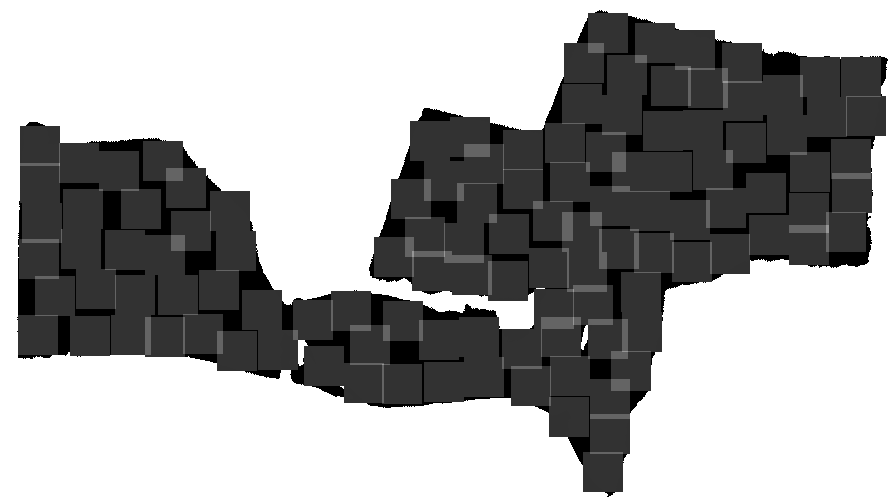
\includegraphics[width=0.475\textwidth]{img/fig13a.png}}\qquad
%   \subfloat[Coverage path planning for 99.71\% of coverage with a distance of 4785px.]{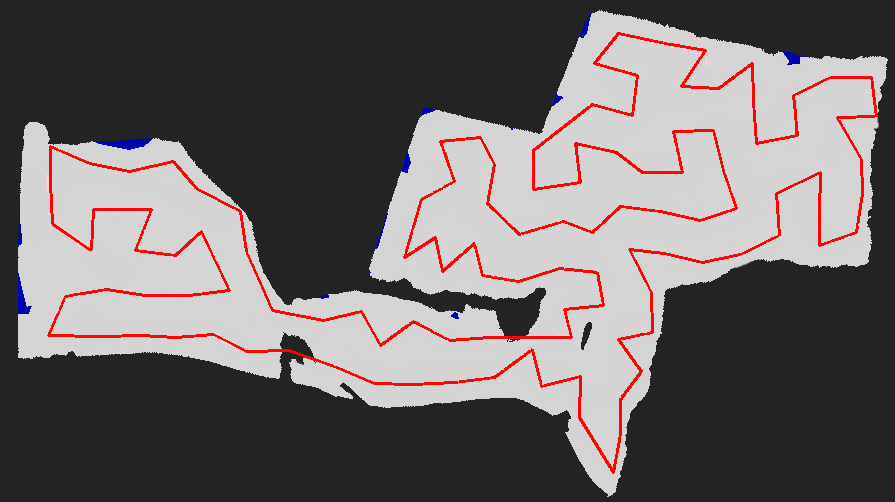
\includegraphics[width=0.475\textwidth]{img/fig13b.png}}\hfill
%   \subfloat[][]{}  
%  \caption{Outdoor simulation of the coverage path planning. The camera projection FOV is $40 \times 60 px$  and fix altitude(with  a scare projection of 40px wild for the positioning optimisation).}\label{fig:trajectoryPathHolo} 
%\end{figure}



  \begin{mfigures}[!]{Outdoor simulation of the coverage path planning. The camera projection FOV is $40 \times 60 px$  and fix altitude(with  a scare projection of 40px wild for the positioning optimisation).}{fig:CalvissonPathPlan} \centering
%\mfigure{width=.4\linewidth}{img/room_python.PNG}{Poses of every image captured in the room}{subfig:RoomPy}
\mfigure{width=.4\linewidth}{img/fig14-a.png}{110 waypoints for $88.38\%$ of coverage
fix altitude .}{subfig:CalvitfullRoomPathHolonom}
\hspace{1cm}
\mfigure{width=.4\linewidth}{img/fig14-b.jpg}{Path planing using the pattern
method Coverage path planning for 98.6\% of coverage with a distance of 8114px.}{subfig:CalviPathPlanningHolonom}
\tabsimuposeCalviPathHolonom
\end{mfigures}  
% \subsubsection{Non holonomic robot2.}
% 
% The next step to estimate the final coverage of the area with the camera stream and the
%UAV trajectory is to orient the cameras depending then the trajectories (see Figure
%14(b)). Obviously the final coverage path planning is better than the estimation
%did it during the waypoint positioning in the following example Figure 14(a).
%The camera projection is 70 pixel by 70 pixel with 110 waypoints for waypoints 
%coverage estimation of 88.38% and 98.64% for the full room after the simulation
%of path planning ((see Figure \figref{subfig:CalvitfullRoomPathHolonom} 14(b)). This gain in not taken into account during
%the phase of estimation numbers of the waypoints (section 3.4). This experiment
%demonstrates by one example the ability of our proposition to do coverage path
%planning in a large area with a non convex shape with different constraint.
% 
%  \begin{mfigures}[!]{Outdoor simulation of the coverage path planning. The camera projection FOV is $40 \times 60 px$  and fix altitude(with  a scare projection of 40px wild for the positioning optimisation).}{fig:CalvissonPathPlan} \centering
%%\mfigure{width=.4\linewidth}{img/room_python.PNG}{Poses of every image captured in the room}{subfig:RoomPy}
%\mfigure{width=.4\linewidth}{img/fig14-a.png}{110 waypoints for $88.38\%$ of coverage
%fix altitude .}{subfig:CalvitfullRoomPathHolonom}
%\hspace{1cm}
%\mfigure{width=.4\linewidth}{img/fig14-b.jpg}{Path planing using the pattern
%method Coverage path planning for 98.6\% of coverage with a distance of ???px.}{subfig:CalviPathPlanningHolonom}
%\tabsimuposeFleyPathHolonom
%\end{mfigures}  

\section{CPP global optimization attempt}

The experiments made previously were successful despite the different optimization steps. In fact to can compute an efficient CPP several optimization has been used (see example Section \ref{sec:experiment}). %with an increasing number of waypoints until reaching an acceptable threshold of coverage rate (see Section \ref{sec:NonEAmethod}).
First number of waypoints has to be estimated and the waypoints poses has to be optimised. When the coverage rate is reached the optimized waypoints can be refined with a PSO to have an appropriate coverage. The final optimization is to use the TSP paradigm to compute a path passing by all the waypoints (as explained in Section \ref{sec:CPPsequantielMethod}). % The estimation of the number of waypoints appear as the most consumer of computation but the case shown during the experimentation the number of waypoints was fixed manual.% (due to the knowledge about each map). 
Despite the success of this greedy method a logical improvement clue maybe to reduce the number of successive optimization. In the experiments proposed previously the waypoints positioning optimization shown some beginning of limit due to the too hight number of dimensions to optimize (see Section \ref{sec:waypointPoseLimite}). 
In the experiment made for a camera constrain by the UAV trajectory (see Section \ref{sec:holonomie path}), the streamed coverage area increase significantly compared to the waypoint coverage. This increased area covered is not taking in account until now. The idea is to try to limit the number of waypoints by using a global method to optimize the CPP problems.\\
The method explored in the following section is to merge the optimisation of the waypoints positioning and the sorted waypoints process to have only one global optimization for the CPP problem. 
 
		\subsection{Adapted formulation }
In order to find a solution for the problem of CPP, by one optimization of the waypoints positioning and the path planning, the problem has to be re-adapted.
Until now, the waypoints positioning and the path planning computation were made by using 2 different GA during 2 different optimizations process. The idea here is to combine the cost function from the waypoints positioning and the path planning computation to have an appropriate and global cost function.
To create this cost function few things are necessary.
\begin{itemize}
	\item First is to estimate the area covered. The area has to take in account not only the area covered by each waypoints but also the covered area during the path (stream coverage). In contrary then the coverage estimation used in the previous section with are discretized (only at each waypoints). %In this case the area covered as to be take in account in continue during all the path.
	\item Second is the path distance. The path distance was already used to estimate the path passing  by all the given waypoints during the path computation (as in Section \ref{sec:TSP2}). In this case that imply to have beforehand the sorted waypoints for the path.
\end{itemize}

\paragraph*{Coverage path plan estimation}\label{par:CPPestimation}

  \begin{mfigures}[!]{Covered area between waypoints following the path plan. Where $Wr$ and $Hr$ are the size of the camera projection  as defined in the Section \ref{sec:coverageEstimation}.}{fig:coverageCPP} \centering
%\mfigure{width=.4\linewidth}{img/room_python.PNG}{Poses of every image captured in the room
\mfigure{width=.8\linewidth}{img/CoverageCPP1.png}{}{subfig:AAA}

\end{mfigures}  



To formulate properly the CPP problem is essential to can estimate the area covered by the UAV during the path passing by all the optimized waypoints. For that the waypoints and the path must be knew. 
%The area covered by the path planning need to be computed for that path passing by all the waypoints is required.
 Once the path knew the coverage estimation can begin. \\
 The idea is to consider all the points of the grid $G$ (see Section \ref{sec:Grid} for the grid definition) between two waypoints as covered. To can compute the points cover during the fly over two waypoints the camera fixed on the UAV as to be known in term of projection on to the floor and the direction. In fact the size of the camera projection and the direction will change the coverage. The direction is directly deducted from the waypoints positions and the size of the camera projection form the camera parameters as this altitude (see Section \ref{sec:CamerasDefinition}). Based on the projection size onto the floor the area cover between the waypoints are deduced as illustrate in Figure \figref{fig:coverageCPP}.

 
%The camera rolls follow the direction of the line between the two points.
% Concretely the implementation is to first estimate the direction and the trajectory to follow  between the two waypoints, estimate the area covered by the camera projection at regular interval on the trajectory. This  coverage path estimation is made between two point until the path is accomplished (to extend $Pc_i$ as in \ref{eq:Pci}).
 That mean in this case the roll of the camera is not optimized but taken in account depending then the trajectory to follows. Moreover in this case the altitude of the UAV is fixed in order to simplify the optimization computations and simplify the cost function.

The methodology proposed to estimate the area covered by the path require to have a set of waypoints ordered.  In the previous algorithms the TSP paradigms with a GA optimisation was used to order the waypoints to have the shorter path passing by the set of optimized waypoints. In this new method, the path as to be compute in the same optimization then the waypoints positioning. 
To do that the solution is to priories the chromosomes order (or particles). The idea is to use the position of each each genome inside the chromosome as important in the estimation. Where in this case a genome is the set of parameters of a waypoint. That mean the same genome at different position has not the same impact in the cost function. Consequently the optimization is not only focus on finding the best coverage for a set of waypoints but also find the sequence of waypoints position. This formulation add some combinator constraint inside each chromosomes and particle.
To illustrate an example is provided in the Figure \figref{fig:orderedK} : \\
The solution ABCD (see Figure \figref{subfig:orderKABCD}) where A; B; C and D are the optimized positions of the waypoints and another solution  ABDC (see Figure \figref{subfig:orderKABDC}) which has found the same waypoints but not in the same order. In the precedent proposed method only the coverage at each waypoint was used to estimate the coverage. Therefore the cost function estimate the 2 solutions as identical. 
In this new estimation of the coverage by taking in account not only the coverage of a set of waypoint but the entier path plan coverage the order of the position give the path to follow. Consequently the solutions are completely different, ABCD (see Figure \figref{subfig:orderKABCD}) is much better due to this shorter path for the equivalent coverage.
  \begin{mfigures}[!]{}{fig:orderedK} \centering
%\mfigure{width=.4\linewidth}{img/room_python.PNG}{Poses of every image captured in the room
\mfigure{width=.4\linewidth}{img/pathPlanOrdred1.png}{ABCD}{subfig:orderKABCD}
\mfigure{width=.4\linewidth}{img/pathPlanOrdred2.png}{ABDC}{subfig:orderKABDC}
\end{mfigures}   

 Finally the new cost function will integrate the covered area by the path passing  by all the waypoints and the distance of this path. The goal is to have a cost function appropriate to maximize the area covered with the shorter path at same time.
 The cost function dedicated to quantify the CPP for the optimization of waypoints positioning and path planning is :
 
  \begin{equation} \label{eq:CostF2}
f=\sum_{i=1}^{n}Pc_i + \frac{\sum_{i=1}^{n}Pc_i}{(\frac{Distance}{N})\times 10}  
\end{equation}  
Where $\sum_{i=1}^{n}Pc_i$ is the number of points cover by the path plan (as discussed in the paragraph \ref{par:CPPestimation} and  Section \ref{eq:Pci}) and the $Distance$  is  the size of the path. The $0.5$ is an empirical coefficient to minimize a bite the distance importance in favour to the coverage.



\paragraph*{Optimization}
 Once the answer quality evaluate thanks to this redefined cost function, it is time to discuses about the optimization process.
One more time the GA is used associate to the PSO. If the EA (especially the GA) are used here is for few main reasons. The GA was the best algorithms to solve the TSP problem and also well adapted to the waypoints positioning (even more with an GAPSO). The last reasons are the knowledge grab about the GA PSO until know make the implementation fast and easy.
 The solution adopted is to use the GAPSO as introduced in \ref{sec:hybridGAPSO} associate to the newly adapted cost function (see Paragraph \ref{par:CPPestimation}).


		\subsection{Result  and consequences }
\begin{mfigures}[!]{Path plan for maximize the covered area with an cameras projection  equal to 40x60. The area is covered  with 5 and 8 waypoints}{fig:TorCPP} \centering
\mfigure{width=.4\linewidth}{img/Tor2bisMapCPPGAcouv0_590046Dist818_306718cam5bis.png}{Distance 818.31px for 5 Waypoints.}{subfig:CPPTorcymapGA}
\hspace{1cm}
\mfigure{width=.4\linewidth}{img/Tor2bisMapCPPGAPSOcouv0_547956dist936_605123cam5bis.png}{Distance 936.61px for 5 waypoints.}{subfig:CPPTorcymapGAPSO}

\mfigure{width=.4\linewidth}{img/Tor2bisGAcouv0_65Dist972_89cam8.png}{Distance 972.89px for 8 Waypoints.}{subfig:CPPTorcymapGACam8}
\hspace{1cm}
\mfigure{width=.4\linewidth}{img/Tor2bisGAPSOcouv0_65Dist972_89cam8.png}{Distance 1101.64px for 8 waypoints.}{subfig:CPPTorcymapGAPSOCam8}
\end{mfigures}
		
		
	Based on the new problems formulation and the use of an appropriate GAPSO directly inherited then the waypoints positioning (see Chapter \ref{chap:waypointPoseExp}) few experiments has been made. The experiments proposed here is based on the map presented in the Section \ref{sec:maskGAPSO}.
% The experiment flow: 
  Once the map selected the optimization begin with 3 waypoints  and the number of waypoints is slightly increased until reach 9 waypoints. For each number of waypoints  3 optimizations has been made. The experiment proposed in the Figure \figref{fig:TorCPP} are the interesting and representatives then the experiments made. 

	\paragraph*{Experiment and discussion}	
The experiment made allows to see the advantage and limit of this optimisation. 
The main advantage of this formulation is the beside to optimize the CPP problem in one unique optimisation is the reducing amount of waypoint compared to the waypoint positioning optimization. In fact for the map proposed only  5 waypoints are required to cover  the area (see Figure \figref{subfig:CPPTorcymapGAPSO}) compare then the waypoints positioning optimisation require 25 waypoints (see Figure \figref{subfig:coverageGAPSOTorcy}). Reducing the number of waypoints needed to cover an area is essential to have an better and faster optimization process. The reducing amount of the number of waypoints is even more important when the problem is complicated by the position order of the waypoints in a solution. 
	On the other side, despite a good coverage of the area the path plan appear too long with many overfly (overlap). Consequently, and despite the good  coverage the path appear not so well optimized. 
	About the optimization we can observe the average numbers of generation of the GA required is around 47 generation for a set of experiment between 3 to 9. The average number of generation is  comparable to the number of generation needed to optimize the waypoints positioning ( see in Section \ref{sec:maskGAPSO}), where for 25 waypoints to pose estimate 67 generation was needed. 
	The fast studies of these experiments, show some limit of using the unique optimization for the problem of CPP. In the other hand, the formulation despite the inconclusive, but promising result appear interesting and the cause of the inconclusive result are explored.
	
	\paragraph*{Why inconclusive result?}
			  
		
		Despite inconclusive results during the first experiments made, it is an interesting track to follow  which must  be more explored.  
		The inconclusive result of the experiment can be from : %the algorithms used, the cost function or the increased complexity and search space size.
		\begin{itemize}
		\item The algorithms: As that was introduced the GAPSO  with a similar set-up than the previous experiment for the waypoints positioning (see Chapitre \ref{chap:waypointPoseExp}) are used. Few inconclusive tests have been done to slightly modify the set-up of the GAPSO by adding more mutation for example. The inconclusive preliminary result push to consider the GAPSO proposed previously good enough and the other reason has to be explored.
		\item The cost function: The cost function presented in the Equation \ref{eq:CostF2} is the more appropriate due to our experiments. Despite that the cost function has some coefficient which they were found empirically. The coefficient could be an interesting track which must be thorough in order to reduce their uncertainty.
		\item Complexity and search space: 
		The last potential reason of the inconclusive result obtained can be the increased size of the search space and complexity. The size of the search space was discussed in the Section \ref{sec:OptimizationComplexity}. The search space estimation was made for the problem of optimizing the waypoints positions and can be reused by part for the problem of CPP for a unique optimization. First the Equation \ref{eq:SearchSpace} can be simplified.  
		\begin{equation} \label{eq:SearchSpaceCPP}
		 Sp=(W\times H)  
		\end{equation}
		Where $W$ and $H$ are the size as width and height of the area to cover. $Sp$  is simplified due to the reduced number of dimension optimized. In fact the altitude is fixed and identical for all the waypoints as the pant and tilt. Regarding the roll depend then the path plane.
		Despite the important decreasing of a search space for each waypoint ($Sp$), the global search space for the CPP increase dramatically  due to the number of waypoint and  the ordered constraints. In fact due to the ordered constraints and the  global search space is re-defined as :
		\begin{equation} \label{eq:ArrangmentCPP}
			A^{Sp}_{N}=\frac{Sp!}{(Sp-N)!} = |Vs|
		\end{equation}
 Where $|Vs|$ is the number of possible solution for a set of $N$ cameras. Due to the importance of the waypoints order in the optimization process the number of possible solution increase greatly. Obviously due to the complexity of the problem and the increased size of the global search space for CPP problem  can be one of the important reason of the inconclusive result.
 \end{itemize}
		
The conclusion is despite the low quality of the answer obtained with these methodologies the interesting track and possible gain must push the research to continue to explore the GAPSO optimization to solve the problem of coverage path planning problem as a one optimization problem. But caution the increased search space can become break of the optimization despite the reducing of the number of dimensions to optimize. In fact, the number of dimensions is reduced by fixing the altitude and the camera orientation and moreover with this  unique optimization  the number of required waypoints are greatly reduced. 
The main risk of using  a unique optimization for the problems of CPP is the complexity and the associate search space. In fact, among the reason to explain the inconclusive results, the complexity due to the fusion of 2 NP-hard and NP-complete problems could be the cause. \\
		


%%%%%%%%%%%%%%%%%%%%%%%%%%%%%%%%%%%%%%%%%%%%%%%%%%%%



